\documentclass[sigconf]{acmart}

% A4 instead of letter paper
\geometry{a4paper}

\usepackage[babelshorthands]{polyglossia}
\setdefaultlanguage[babelshorthands=true]{german}
\usepackage[autostyle=true, german=quotes]{csquotes}
\usepackage{booktabs} % More formal table style.
\usepackage{xcolor}

% ACM style ``tweaking''
\settopmatter{printacmref=false}                   % Removes citation information below abstract
\renewcommand\footnotetextcopyrightpermission[1]{} % Removes footnote with conference information in first column
\pagestyle{plain}                                  % Removes running headers

% Code
\definecolor{light-gray}{gray}{0.95}
\newcommand{\code}[1]{\colorbox{light-gray}{\texttt{#1}}}

% Figures
%\DeclareGraphicsRule{.ai}{pdf}{*}{}% Handle .ai files as .pdf files.
%\DeclareGraphicsExtensions{.pdf,.ai,.jpg,.png}
%\pdfpagebox 5% Use ArtBox instead MediaBox. 1=MediaBox, 2=CropBox, 3=BleedBox, 4=TrimBox, 5=ArtBox. (shell: pdfinfo -box <pdf-file>)
%\setkeys{Gin}{pagebox=artbox}% Alternative (necessary for newer tex versions) for \pdfpagebox 5 in preceding line.
\graphicspath{{../report-ufo-figures/}}

%\usepackage[backend=biber]{biblatex}
%\addbibresource{report-ufo.bib}


\usepackage[math]{blindtext} % TODO Remove after adding own content.
\usepackage{hyperref}

\begin{document}

\title{Bericht der Gruppe \glqq Ufo\glqq}
\subtitle{Eine Analyse der Abhängigkeit der Wetters auf vermeintliche Ufo-Sichtungen.}         % Optional.

\keywords{Übung {\glqq Big Data Analytics\grqq}, Sommersemester 2021, Ufo}

\author{Lars Thomsen, Uzeyir Mammadov}
\affiliation{%
    \institution{%
        Martin-Luther-Universität Halle-Wittenberg
    }
}
\email{[lars.thomsen][uzeyir.mammadov]@student.uni-halle.de}

\begin{abstract}
 Some general hints on what to mention in an abstract: What are the questions you address? Why are they interesting? What approaches did you use? What answers did you find?
 
 As for how to structure the abstract: Give some motivation and context on the general topic you address (1--2~sentences). Then state the specific questions you address (1--2~sentences) and describe how you approach them (2--3~sentences). Finally, results and some conclusion (1--3~sentences).
\end{abstract}

\maketitle

\section{Einleitung} \label{einleitung}

Auf den ersten Blick klingen vermeintliche Ufo-Sichtungen immer nach an den Haaren herbeigezogenen Erfindungen und Lügengeschichten. Doch wie viel Wahrheit steckt in diesen Sichtungen, und lassen sich gegebenenfalls Muster in diesen erkennen?

% Welchen Einfluss nimmt das zum Zeitpunkt der Sichtung herrschende Wetter auf die Sichtung von vermeintlichen Ufos?
Im Zuge unseres Projektes haben wir uns folgende Forschungsfrage gestellt: Existieren Abhängigkeiten zwischen vermeintlichen Ufo-Sichtungen, und welchen Einfluss nimmt das zum Zeitpunkt der Sichtung herrschende Wetter?

Als Grundlage dafür dienen uns ein Datensatz des \enquote{National UFO Reporting Center} (NUFORC)\cite{nuforc:2021} sowie Wetterdaten für Vergleiche und Analysen von Meteostat\cite{meteostat:2021}.

Der Bericht gliedert sich wie folgt: Kapitel \ref{data} beschreibt die verwendeten Daten und Datensätze. In Kapitel \ref{versuch1} werden die ersten Versuche kurz erklärt, bevor in Kapitel \ref{forschungsfrage} die Forschungsfrage und ihre Bearbeitung vorgestellt wird. Kapitel \ref{evaluation} diskutiert die Ergebnisse unserer Frage. Im Schlusskapitel (\ref{fazit}) geben wir unser Fazit und runden den Bericht ab.

\begin{figure}[t]
    \centering
    
\includegraphics[width=\columnwidth]{nuforc_logo}
    \caption{NUFORC.}
    \label{fig:nuforc}
\end{figure}
\section{Daten} \label{data}

Die verwendeten Datensätze stammen aus einer Datenbank vom \enquote{National UFO Reporting Center} (NUFORC). In diese Datenbank kann jede Person ihre vermeintliche Ufo-Sichtung -- entweder online über ein Formular oder per Telefon -- eintragen. Des Weiteren senden gewisse Messstationen, zum Beispiel MADAR Nodes, auffällige Messdaten automatisch an die Datenbank\cite{madar:2020}. Da die zur verfügung stehenden Daten für das Projekt keinen Mehrwert baten, wurden diese nicht beachtet. Um offensichtlichen Fakes entgegenzuwirken werden die eingereichten Daten vor der monatlichen Veröffentlichung von den Betreibern des Portals überprüft.

Jeder Eintrag des Datensatzes besteht aus dem Datum und der Uhrzeit der Sichtung, der Stadt sowie dem Kürzel des dazugehörigen Bundesstaates (ausschließlich für die USA), einer klassifizierten Beschreibung der Form des Ufos und gegebenenfalls einer kurzen Zusammenfassung und Beschreibung aus der Sicht des Einsenders.

Für diese Daten haben wir eine einfache Datenbank erstellt, um auch offline auf diese zugreifen zu können. Um die Daten einfacher verarbeiten zu können, bereiten wir diese während der Abfrage von unserer Datenbank auf und treffen eine Vorauswahl an brauchbaren Daten. Die Kriterien für die Vorauswahl wurden durch stichprobenartige Abfragen festgelegt. Dem entsprechend werden Einträge von vorhin beschriebenen externen Messstationen, Einträge mit fehlenden Inhalten oder \enquote{?} als Inhalt nicht betrachtet. Der Datentyp aller Attribute ist der Einfachheit halber nur string. Zu einem späteren Zeitpunkt werden Datum und Uhrzeit in ein datetime-Format überführt. Mit dem Wissen aus den stichprobenartigen Abfragen legen wir uns auf die zwei gängigsten Formate fest -- 'm/d/y H:M' und 'm/d/y'. Andere in dem Datensatz vorkommenden Formate oder von den Einsendern eigenständige Angaben beachten wir nicht. Die aufbereiteten Daten werden letztendlich durch das Tripel \code{datetime}, \code{city} und \code{state} beschrieben.

Als Quelle für die Wetterdaten haben wir uns letztendlich für \enquote{Meteostat} entschieden\cite{meteostat:2021}. Auf diese Daten wird über die dazugehörige Python-Library zugegriffen. Essenziell für unser Projekt sind die Attribute \code{tsun} (Anzahl der Sonnenminuten) und \code{coco} (Klassifizierter Zustand des Himmels). Die Daten sind für unsere Vorhaben bereits von ausreichender Qualität, sodass in diesem Fall keine weitere Aufbereitung und Säuberung der Daten nötig ist.

\begin{table}[t]
    \caption{Kennzahlen des Datensatzes.}
    \label{tab:data}
    \centering
    \small
    \begin{tabular}{l r}
        \toprule
        Einträge & Anzahl\\
        \midrule
        Gesamt & 96~924\\
        Davon einzigartige Orte & 25~234\\
        \midrule
        Orte mit Wetterdaten, gesamt & 2~020\\
        Davon mit Sonnenminuten pro Stunde & 26\\
        Davon mit Sonnenminuten pro Tag & 116\\
        Davon mit condition codes & 1~886\\
        \bottomrule
    \end{tabular}
\end{table}
\section{Die ersten Versuche} \label{versuch1}  % Change title accordingly

Die erste Idee war es, die Wetterdaten für unsere Forschungsfrage von den \enquote{National Centers for Enviromental Information} (NCEI) zu beziehen. Diese Datensätze beinhalten für unsere Analyse zwei wesentliche Attribute: \code{HourlySkyCondition} und \code{HourlyVisibility}. Diese beiden Werte beschreiben zum Ersten den klassifizierten Zustand des Himmels (z.B. Regenwolken, Schleierwolken, Nebel etc.) und zum Zweiten die prozentuale Bedecktheit des Himmels. Die Liste aller verfügbaren Stationen sind ebenfalls beim NCEI verfügbar(Link Stationen).

Um die Daten einer Ufo-Sichtung mit den dazugehörigen Wetterdaten zu verknüpfen, wird das jeweilige eindeutige \code{city, state}-Tupel der am nahestehendsten Wetterstation zugeordnet. Um die Ergebnisse nicht zu sehr zu verfälschen, wurde das zulässige Einzugsgebiet einer Wetterstation auf 20 Kilometer, mit der Station als Zentrum, begrenzt.

Diese Idee konnte leider nicht umgesetzt werden. Es standen zwar zwei Versionen der API vom NCEI zur verfügung, allerdings greifen diese auf unterschiedliche Stationen zurück. Dabei waren zwei Probleme die Hauptursache für das Aufgeben dieser ersten Idee: Zum Ersten waren die internen Bezeichnungen der Stationen bei Version~1 der API verschieden zu denen der uns zur verfügung stehenden Liste. Eine einheitliche Liste aller Stationen, welche durch Version~1 der API bedient werden war nicht verfügbar. Zum Zweiten wurde von Version~2 der API eine verschiedene zur bereits verarbeiteten Liste an Stationen verwendet, welche nur unter Umständen einsehbar war. Somit war es nicht möglich mit den verwendeten Datensätzen die gestellte Forschungsfrage zu bearbeiten.
\section{Forschungsfrage} \label{forschungsfrage}

Test
\section{Evaluation} \label{evaluation}

Die Bearbeitung der Forschungsfrage hat folgende Ergebnisse hervorgebracht: Aus ursprünglich 96~924 potenziell relevanten Ufo-Sichtungen im Datensatz konnten für 2~020 Sichtungen zu dem Zeitpunkt passende Wetterdaten gefunden werden, das entspricht ungefähr 2,1\%. Mit welcher Art der drei Vergleichsdaten die Sichtungen analysiert wurden lässt sich in Tabelle \ref{tab:data} ablesen.

\begin{figure}[t]
    \centering
    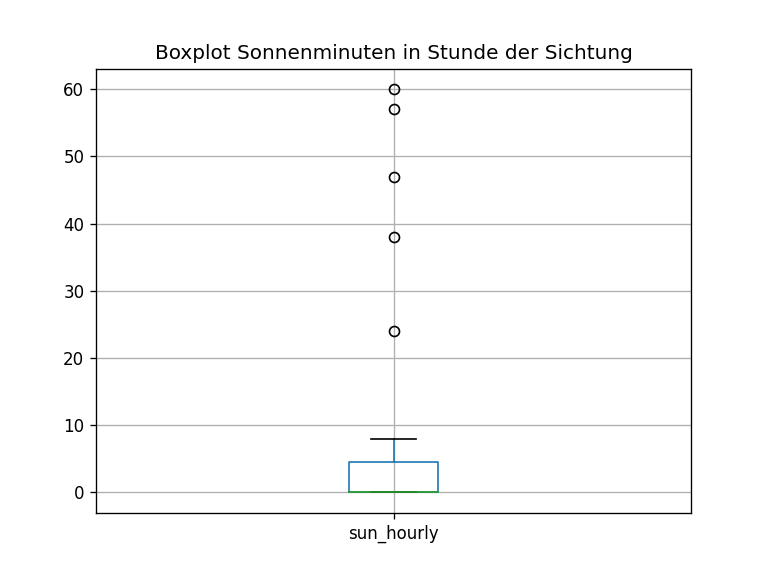
\includegraphics[width=\columnwidth]{hourly_suntime_boxplot}
    \caption{Sonnenminuten pro Stunde.}
    \label{fig:hourly_suntime}
\end{figure}

Die Vergleichsdaten mit dem am Abstand wenigsten Vorkommen bilden die Sonnenminuten pro Stunde mit lediglich 26 Einträgen. Wie in Abbildung \ref{fig:hourly_suntime} zu erkennen ist, befindet sich die Mehrheit davon im Bereich von 0 bis 5 Sonnenminuten pro Stunde. Vereinzelte Ausreißer reichen gegen 50 bis 60 Sonnenminuten.%Aufgrund der sehr geringen Datenmenge und der Erkenntnis, dass es sich bei fast allen Werten um \enquote{0 Minuten} handelt,  

\begin{figure}[t]
    \centering
    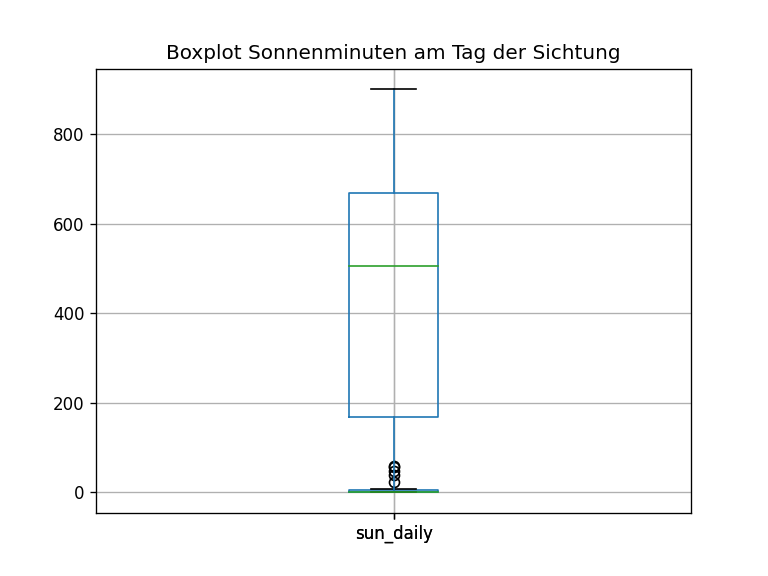
\includegraphics[width=\columnwidth]{daily_suntime_boxplot}
    \caption{Sonnenminuten pro Tag.}
    \label{fig:daily_suntime}
\end{figure}

Abbildung \ref{fig:daily_suntime} beschreibt die Verteilung der Sonnenminuten pro Tag an jeder verfügbaren Ufo-Sichtung. Die mittleren 50\% der Ergebnisse sind hierbei, im Gegensatz zu den stündlichen Sonnenminuten, breiter verteilt. Sie reichen von 200 bis 700 Sonnenminuten pro Tag mit wenigen Ausreißern, welche nur gegen weniger Minuten streben. Im Schnitt scheint die Sonne während eines Tages, an dem ein vermeintliches Ufo gesichtet wurde, um die 500 Minuten -- also etwas mehr als 8 Stunden. In Anbetracht dessen, dass die durchschnittlichen Sonnenstunden in den USA im Bereich zwischen 2 Stunden im Winter und bis zu 12 Stunden im Sommer reichen, kann man den Ufo-Sichtungen eine leichte Überdurchschnittlichkeit an Sonnenstunden zuordnen\cite{statista:2021}.

\begin{table}[t]
    \caption{Condition Codes.}
    \label{tab:coco}
    \centering
    \small
    \begin{tabular}{l l r}
        \toprule
        Code & Weather Condition\cite{coco:2021} & Anzahl\\
        \midrule
        0 & - & 15\\
        1 & Clear & 227\\
        2 & Fair & 603\\
        3 & Cloudy & 363\\
        4 & Overcast & 93\\
        5 & Fog & 186\\
        7 & Light Rain & 219\\
        8 & Rain & 51\\
        9 & Heavy Rain & 9\\
        12 & Sleet & 1\\
        14 & Light Snowfall & 42\\
        15 & Snowfall & 2\\
        16 & Heavy Snowfall & 1\\
        17 & Rain Shower & 9\\
        18 & Heavy Rain Shower & 23\\
        25 & Thunderstorm & 35\\
        26 & Heavy Thunderstorm & 5\\
        27 & Storm & 2\\
        \bottomrule
    \end{tabular}
\end{table}

\section{Conclusion} \label{conclusion}

The introduction in less detail. Summarize story in retrospective, give outlook on possible next steps. Semi-technical \ldots


%\bibliographystyle{ACM-Reference-Format}
%\printbibliography

\end{document}
